% LoRA vs ReFT visual: weight-space adapters vs representation edits
\documentclass[tikz,border=5pt]{standalone}
\usepackage{xcolor}
\usepackage{fontspec}
\usetikzlibrary{arrows.meta,shapes.geometric,fit,shadows.blur,positioning}

% Define color scheme
\definecolor{primaryblue}{RGB}{41,128,185}
\definecolor{secondarygreen}{RGB}{39,174,96}
\definecolor{accentorange}{RGB}{230,126,34}
\definecolor{warningred}{RGB}{231,76,60}
\definecolor{lightgray}{RGB}{236,240,241}
\definecolor{darkgray}{RGB}{52,73,94}

\begin{document}
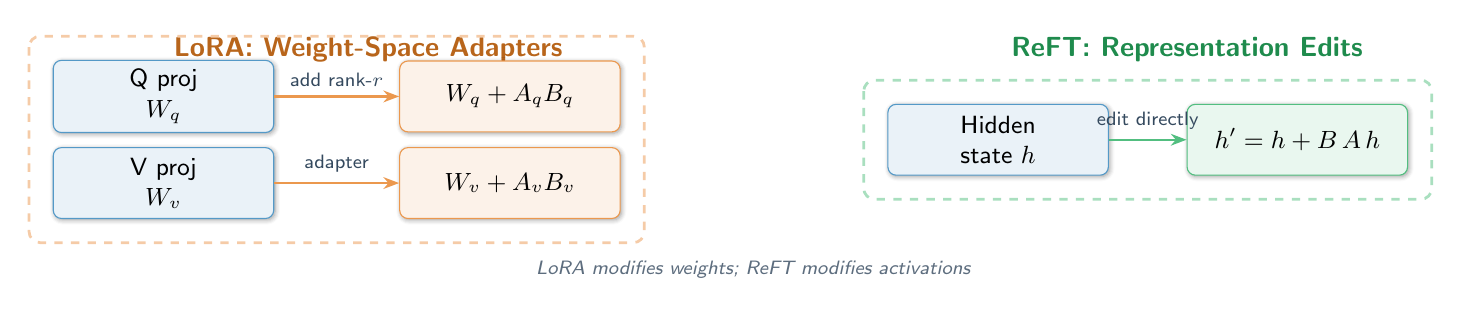
\begin{tikzpicture}[
  node distance=10mm and 16mm,
  block/.style={
    draw=primaryblue!80,
    fill=primaryblue!10,
    rounded corners=3pt,
    minimum width=28mm,
    minimum height=9mm,
    align=center,
    font=\sffamily\small,
    blur shadow={shadow blur steps=5, shadow xshift=0.5pt, shadow yshift=-0.5pt}
  },
  lorablock/.style={
    draw=accentorange!80,
    fill=accentorange!10,
    rounded corners=3pt,
    minimum width=28mm,
    minimum height=9mm,
    align=center,
    font=\sffamily\small,
    blur shadow={shadow blur steps=5, shadow xshift=0.5pt, shadow yshift=-0.5pt}
  },
  reftblock/.style={
    draw=secondarygreen!80,
    fill=secondarygreen!10,
    rounded corners=3pt,
    minimum width=28mm,
    minimum height=9mm,
    align=center,
    font=\sffamily\small,
    blur shadow={shadow blur steps=5, shadow xshift=0.5pt, shadow yshift=-0.5pt}
  },
  line/.style={-{Stealth[length=2mm]}, thick, draw=darkgray},
  loraline/.style={-{Stealth[length=2mm]}, thick, draw=accentorange!80},
  reftline/.style={-{Stealth[length=2mm]}, thick, draw=secondarygreen!80},
  annot/.style={font=\sffamily\scriptsize, text=darkgray},
  title/.style={font=\sffamily\bfseries, text=darkgray}
]

% ===== Left side: LoRA (weight-space) =====
\node[title, accentorange!80!black] at (26mm,6mm) {\textbf{LoRA}: Weight-Space Adapters};

% LoRA blocks
\node[block] (wq) at (0,0) {Q proj\\$W_q$};
\node[block] (wv) at (0,-11mm) {V proj\\$W_v$};
\node[lorablock] (wq_lora) at (44mm,0) {$W_q + A_q B_q$};
\node[lorablock] (wv_lora) at (44mm,-11mm) {$W_v + A_v B_v$};
\draw[loraline] (wq) -- (wq_lora) node[midway, above, annot] {add rank-$r$};
\draw[loraline] (wv) -- (wv_lora) node[midway, above, annot] {adapter};

% LoRA box
\draw[draw=accentorange!40, line width=1pt, rounded corners, dashed]
  ($(wq.north west)+(-3mm,3mm)$) rectangle ($(wv_lora.south east)+(3mm,-3mm)$);

% ===== Right side: ReFT (representation-space) =====
\node[title, secondarygreen!80!black] at (130mm,6mm) {\textbf{ReFT}: Representation Edits};

% ReFT blocks
\node[block] (h) at (106mm,-5.5mm) {Hidden\\state $h$};
\node[reftblock] (reft) at (144mm,-5.5mm) {$h' = h + B\,A\,h$};
\draw[reftline] (h) -- (reft) node[midway, above, annot] {edit directly};

% ReFT box
\draw[draw=secondarygreen!40, line width=1pt, rounded corners, dashed]
  ($(h.north west)+(-3mm,3mm)$) rectangle ($(reft.south east)+(3mm,-3mm)$);

% Add comparison annotation at bottom
\node[align=center, font=\sffamily\scriptsize, text=darkgray!80] at (75mm,-22mm)
  {\textit{LoRA modifies weights; ReFT modifies activations}};

\end{tikzpicture}
\end{document}
